%%%%%%%%%%%%%%%%%%%%%%%%%%%%%%%%%%%%%%%%%%%%%%%%%%%%%%%%%%%%%%%%%%%%%%%%%%%%%%%%%%%%%%%%%%%%%%%%%%%%%%%%%%%%%%%%%%%%%%%%%%%%%%%%%%%%%%%%%
\section{Mobility classification}\label{sec:esnr_mobility}
The previous three applications in this chapter used the Effective SNR in algorithms that configure various network parameters. In this section, I use the Channel State Information (CSI) underlying the Effective SNR model to determine whether a wireless device is moving. Though this application does not directly use the Effective SNR, this primitive provides an important complement to the network-level configuration problems.

In wireless systems, simply knowing whether a device is mobile can improve performance and reliability. For example, recent work of Ravindranath et al.\ \cite{Ravindranath_SensorHints} demonstrated a system that improved 802.11a performance on a mobile phone by selecting between different bitrate adaptation algorithms based on whether the device was moving. When the device is static, they use algorithms that can conduct a fine-grained search of the rate space to choose the optimum bitrate. When the device is moving, they use an algorithm that performs a coarser search, but does a better job of tracking a moving optimum. In their experiments, the fine-grained algorithms performed 10\%--30\% better in static scenarios, while the coarse-grained algorithm performed 25\%--75\% better in mobile scenarios.

Detecting mobility can also be used to enhance reliability in networks that support dynamic topology, such as today's cellular phone networks, enterprise Wi-Fi wireless distribution systems (WDSes), and networks that support relaying mechanisms such as described above. By proactively looking for a better AP or relay when the device starts moving, service quality can be improved and downtime reduced. \xxx{find some references about cell handoff, WDS handoff, etc.}

The implementation by Ravindranath et al.\ detected mobility using the accelerometer in a mobile phone. While this technique is accurate and responsive, it has a few disadvantages. The use of an on-board sensor means that detection can only be performed by the mobile client, and thus requires protocol changes to communicate a device's mobile state to the other endpoint of the link: this solution is not backwards-compatible. Also, this technique can only be implemented on devices that have accelerometers, and requires that this sensor be powered on.

In this section, I explore whether it is possible to classify whether a device is mobile based solely on passively measured RF information. If successful, such an implementation would eliminate all of these drawbacks by requiring no extra hardware and supporting unilateral adoption by either endpoint of the link, including the static device. Ravindranath et al.\ made a preliminary attempt to classify mobility using RSSI, but were not successful. They list three challenges: (1) that RSSI is unstable even for static links in a quiet environment; (2) that RSSI varies by different amounts at different absolute signal strengths, and thus needs to be calibrated; and (3) that RSSI was extremely sensitive to movement in the environment and triggered many false hints. Here, I show that the CSI can overcome these challenges and provide a robust solution.

\subsection{Experimental setup}
I configured a SIMO experiment using a single-antenna laptop as the client device, and eight of the testbed nodes as three-antenna monitors. The client sent 100,000 back-to-back short packets using \mcs{0} (1 stream, 6.5\Mbps), approximately one packet every 200\us for 20\s. This sampling rate is higher than practical for Wi-Fi. In particular, packets sent at slow rates or in batches, can last as long as 4\ms. I thus downsampled the trace from 100,000 packets every 200\us to about 5,000 packets every 4\ms before any of the processing described in the rest of this section.

I ran four experiments to analyze a variety of static and mobile channels. For two experiments, I placed a \emph{static} client in the UW CSE Networking Lab, with students present, but not moving in the room. I next took a trace with \emph{environmental mobility} in which I left the client static, but waved my hand within a few centimeters of the antenna and then walked around the room and opened doors. Finally, I took a \emph{mobile device} trace in which I picked up the laptop and moved it around within a meter of its original location. Chronologically, the traces were taken in the order described within a 10-minute window, with the second static trace taken last.

My goal in this section is to develop a simple classification scheme that can distinguish between these scenarios. In particular, I would like to be able to tell, from RF channel effects alone, whether the device is in a static or mobile channel (with device or environmental mobility). A secondary goal is to distinguish between the two types of mobile channels. Ravindranath et al.\ argued that both of these two goals are difficult, if not impossible, with simple RSSI. I believe that the fine-grained information conveyed by the CSI can overcome these deficiencies.

\subsection{Classifying mobility with RSSI}
I begin by analyzing RSSI variation over time to confirm that it is indeed difficult to distinguish between these four traces. \figref{fig:mobility_rssi} shows the RSSI in dBm measured by one receiver for each scenario. In each plot, the three lines each show the RSSI for one of the three receive antennas. With the typical Wi-Fi noise floor around $-92\dBm$, these graphs show the three antennas for a strong receiver with a Packet SNR around 45\dB.

\begin{figure}[htb]
	\centering
	\subfigure[Static Environment]{
		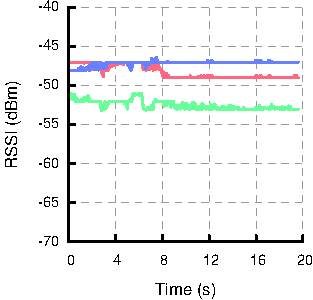
\includegraphics[width=0.43\textwidth]{figures/applications/time_vs_rss_static.pdf}%
	}\hspace{0.06\textwidth}%
	\subfigure[Static Environment, trial 2]{
		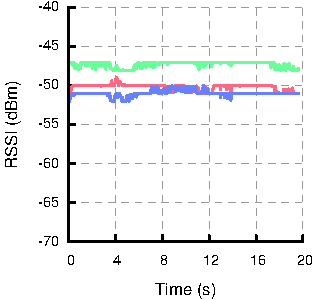
\includegraphics[width=0.43\textwidth]{figures/applications/time_vs_rss_static2.pdf}%
	}
	
	\subfigure[Environmental Mobility]{
		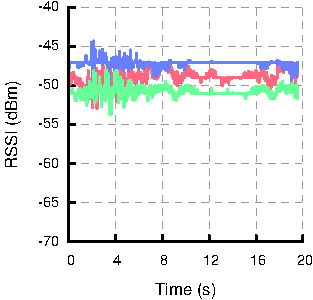
\includegraphics[width=0.43\textwidth]{figures/applications/time_vs_rss_enviro.pdf}%
	}\hspace{0.06\textwidth}%
	\subfigure[Mobile Device]{
		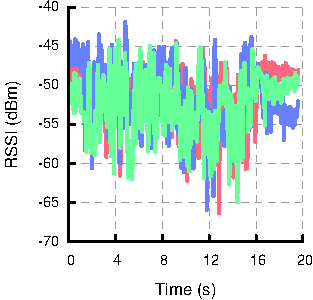
\includegraphics[width=0.43\textwidth]{figures/applications/time_vs_rss_mobile.pdf}%
	}
	\caption{\label{fig:mobility_rssi}RSSI variation in different mobility scenarios.}
\end{figure}

I note several interesting effects visible in these measurements. First, the RSSI is actually extremely stable in static scenarios, varying roughly 2\dB across 20 seconds. This stability deviates from the observations by Ravindranath et al., likely because the newer 802.11n hardware I used is well-calibrated, compared with older 802.11g hardware they used to run experiments with the MadWiFi driver.

Second, though RSSI does vary with environmental mobility, the variation is fairly small and mostly limited to the periods of activity directly next to the client. Later in the trace, when I moved across the room, the RSSI variation decreased to match the static scenario. It also appears that the variation is not completely correlated across antennas; in several parts of this trace (e.g., at the beginning and around 10\s--12\s) one or two antennas see variation in RSSI while the others do not. These periods of partial variation may be indicative of a static device with environmental movement.

Finally, the mobile trace exhibits the RSSI variation with the largest magnitude, and shows consistent variation throughout the trace and across all antennas. This is a dramatic outlier compared to the other traces, and strongly reflects the effects of movement.

Based on this visual evidence, which mirrors the results for the other 7 receivers, I believe it likely that the static scenario actually \emph{can} be identified using RSSI, and hypothesize that it may also be possible to distinguish between environmental and device mobility. However, I deferred exploring these possibility further because, as I will show next, the CSI can conclusively classify a device's activity into these three states.

\subsection{Classifying mobility with CSI}
The last subsection examined the four traces I took---two static traces, one with a fixed device and environmental mobility, and the last with a mobile device---and showed that RSSI variation differs visually across in these four scenarios. Here, I examine the same four traces through the lens of the CSI.

\subsubsection{Quantifying CSI variation: Pearson correlation}
Recall that the RSSI yields a single power measurement for each antenna for every packet, whereas the CSI gives a 3-D matrix of complex numbers that represent magnitude and phase on spatial paths and frequency. To measure the deviation in RSSI, we could simply look at its variation---e.g., absolute difference between samples, or windowed variance---over time, as I showed visually in \figref{fig:mobility_rssi}. In contrast, it is not obvious how to quantify the variation in CSI over time.

I chose a simple method to quantify the variation of CSI, by using the \define{Pearson correlation function} for each spatial path between a transmit-receive antenna pair. The Pearson correlation is the ``standard'' correlation for two $n$-element vectors $\vec{x}$ and $\vec{y}$:
\begin{equation}
\textit{corr}(\vec{x},\vec{y}) = \frac{\sum_{i=1}^n(x_i-\overline{x})(y_i-\overline{y})}{\sqrt{\sum_{i=1}^n(x_i-\overline{x})^2 \sum_{i=1}^n(y_i-\overline{y})^2}}.
\end{equation}
Here $\vec{x},\vec{y}$ are indexed by $i$ and have respective means $\overline{x}$ and $\overline{y}$.

To apply this to CSI, let $\vec{r}_{p,t}$ represent the magnitudes of the CSI coefficients across subcarriers for spatial path $p$ at time sample $t$. Then we can quantify the change between sample $t$ and sample $t+1$ by $\textit{corr}(\vec{r}_{p,t},\vec{r}_{p,(t+1)})$. The correlation will be close to 1 if the CSI matches across time, i.e., the channel is not changing, and closer to zero if the channel varies quickly so that the CSI samples are close to being independent.

\begin{figure}[htb]
	\centering
	\subfigure[Static Environment]{
		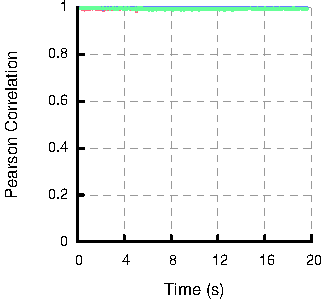
\includegraphics[width=0.43\textwidth]{figures/applications/time_vs_csi_static.pdf}%
	}\hspace{0.06\textwidth}%
	\subfigure[Static Environment, trial 2]{
		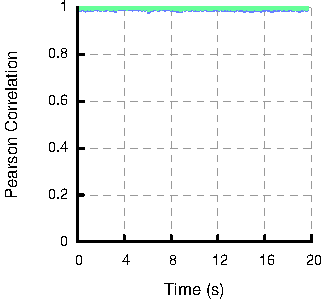
\includegraphics[width=0.43\textwidth]{figures/applications/time_vs_csi_static2.pdf}%
	}
	
	\subfigure[Environmental Mobility]{
		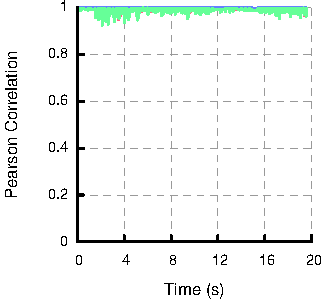
\includegraphics[width=0.43\textwidth]{figures/applications/time_vs_csi_enviro.pdf}%
	}\hspace{0.06\textwidth}%
	\subfigure[Mobile Device]{
		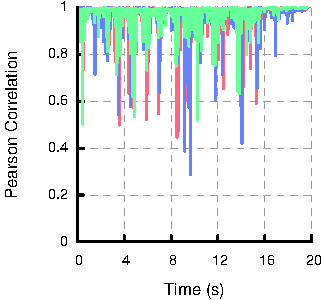
\includegraphics[width=0.43\textwidth]{figures/applications/time_vs_csi_mobile.pdf}%
	}
	\caption{\label{fig:mobility_csi}CSI variation as measured by correlation in different mobility scenarios.}
\end{figure}

\subsubsection{CSI variation results}
Using the same link as in \figref{fig:mobility_rssi}, I present the temporal correlation for the four experiments in \figref{fig:mobility_csi}. Again, each plot shows one line for each of the 3 receive antennas. These plots show that the static traces have near-perfect correlation, close to 1.0 for the full 20\s trace.  In contrast, both the environmental and device mobility traces vary significantly, as low as 0.9 in environmental mobility and 0.3 when the device itself moves. These results thus indicate that the Pearson correlation can classify whether the channel is static, and in changing channel can differentiate whether just the environment is changing or the device itself is moving.

That the environmental and device mobility scenarios exhibit dramatically different correlations might be surprising. To explain this, recall that the frequency-selective channel effects measured by CSI usually result from indoor multipath effects, in which multiple copies of the transmitted signal arrive at the receive antenna after propagating along different (possibly reflected) rays through the RF environment. In many cases of environmental mobility only some of these rays will be affected. If instead the device is itself moving, all paths will be affected. This provides an intuitive explanation for why the temporal correlation is significantly stronger for environmental mobility, though both correlations derivative significantly from the static correlation of 1.

\begin{figure}[tp]
	\centering
	\subfigure[RSSI over time]{
		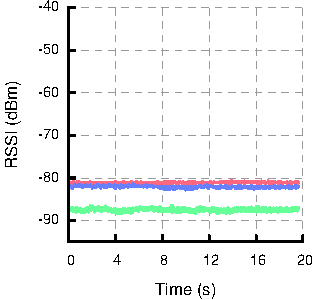
\includegraphics[width=0.45\textwidth]{figures/applications/time_vs_rss_static2_12.pdf}%
	}\hspace{0.03\textwidth}%
	\subfigure[Pearson correlation over time]{
		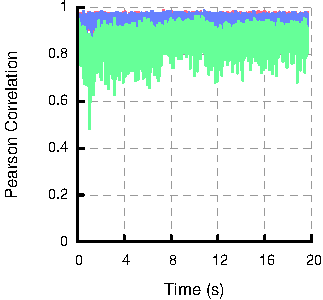
\includegraphics[width=0.45\textwidth]{figures/applications/time_vs_csi_static2_12.pdf}%
	}
	\caption{\label{fig:mobility_example_weak}RSSI and CSI variation for a weak link in a static environment.}
\end{figure}

\heading{CSI correlation for weak links.} 
The Pearson correlation over CSI has thus overcome two of the three drawbacks that Ravindranath et al.\ outlined for classifying mobility using RSSI. First, the correlation of CSI across time is stable for static links. Second, the Pearson correlation can distinguish between environmental mobility and a moving device. The third drawback is that RSSI-based classifiers do not work as well for weaker links: how does my CSI-based classifier perform in this scenario? 

\figref{fig:mobility_example_weak} analyzes the the RSSI and CSI variations during a static trace when the weakest antenna has a Packet SNR of only 5\dB. I found that, indeed, Pearson correlation does not work as well for this weak link. In particular, the correlation against CSI is as low as 0.5, on par with the mobile device for the stronger link shown in \figref{fig:mobility_csi}. The RSSI shown in the left graph also exhibits similarly larger variation for this weak link compared to the strong link analyzed above.

To fix this, I introduced a \define{windowed correlation} scheme. Before computing the Pearson correlation values, I average together 10 consecutive CSI samples. This has the effect of smoothing out the noise corrupting the CSI estimates and restoring the high correlation to the static traces, while only slightly affecting the low correlations for mobile traces.

\begin{figure}[tp]
	\centering
	\subfigure[Windowed CSI correlation for a strong link ($\approx50\dB$ SNR)]{
		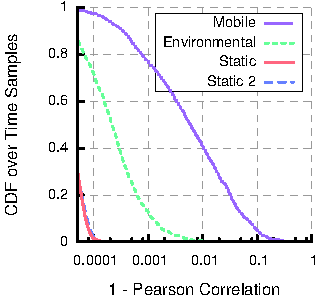
\includegraphics[width=0.45\textwidth]{figures/applications/csi_cdf_link1_10_log.pdf}%
	}\hspace{0.03\textwidth}%
	\subfigure[Windowed CSI correlation for a weak link ($\approx5\dB$ SNR)]{
		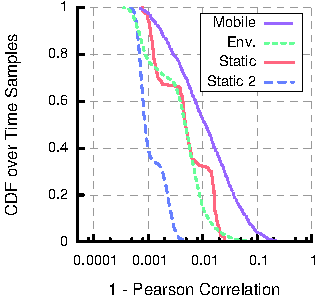
\includegraphics[width=0.45\textwidth]{figures/applications/csi_cdf_link12_10_log.pdf}%
	}
	\caption{\label{fig:mobility_csi_cdf}Windowed CSI variation for a strong and a weak link.}
\end{figure}

\figref{fig:mobility_csi_cdf} shows the CDF of the windowed correlation values (denoted $\mathit{corr}$, and combined across antennas) over time for these same two links. To better illustrate the difference across experiments, I capture the deviation from a perfect correlation of 1.0 by plotting $1-\mathit{corr}$ on a logarithmic scale. Thus a value of 0.001 on the $x$-axis means a correlation of 0.999, while a value of 0.1 means a correlation of 0.9. Recall that lower correlations (right on the graph) imply that the channels are changing faster.

For both the weak and the strong link, the mobile trace stands out. Its line to the right, meaning its correlation is lower, than the other measurements for both links. Focusing on the lowest correlations (the points in the bottom 20\% of each CDF), we can see that only the mobile traces achieve a correlation below 0.9 ($x$-axis value 0.1 or higher). For the stronger link, there is clear separation (at least an order of magnitude) between the mobile trace, the environmental mobility trace, and the static traces. For the weak link, it is difficult to distinguish environmental mobility from the static trace. This indicates that the secondary goal of distinguishing these scenarios may only be achievable for strong links.

\begin{figure}[htbp]
	\centering
	\subfigure[Mobile device]{
		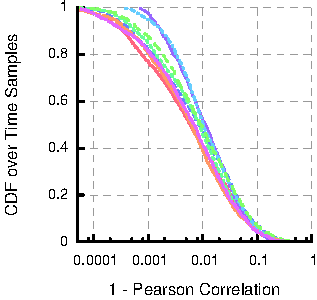
\includegraphics[width=0.3\textwidth]{figures/applications/csi_cdf_mobile_log.pdf}%
	}\hspace{0.03\textwidth}%
	\subfigure[Environmental mobility]{
		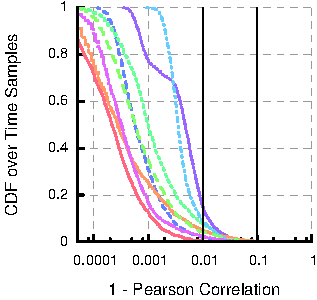
\includegraphics[width=0.3\textwidth]{figures/applications/csi_cdf_enviro_log.pdf}%
	}\hspace{0.03\textwidth}%
	\subfigure[Both static traces]{
		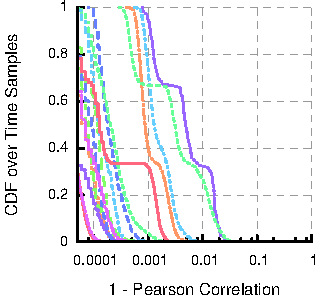
\includegraphics[width=0.3\textwidth]{figures/applications/csi_cdf_static_log.pdf}%
	}
	\caption{\label{fig:mobility_csi_alllinks_cdf}Windowed CSI variation for all eight receivers.}
\end{figure}

\heading{Windowed CSI for all links.} Thus far, I have presented CSI correlation results for one strong and one weak link. Here, I analyze the windowed CSI correlation for each of the three mobility scenarios over all eight of the links. In \figref{fig:mobility_csi_alllinks_cdf}, I present the CDFs of windowed CSI over all eight links, separated into the three mobility conditions scenarios. Note that the mobility and environmental mobility conditions have 8 lines, one for each receiver, while I have combined both static traces into 16 lines on a single graph.

These results show that the features I identified looking at the first two links extend to the entire testbed. Notably, all 8 links exhibit correlations below 0.9 (right of 0.1 on the $x$-axis), while none of the 24 traces in the other two conditions reach this value. For this experiment, my windowed CSI correlation can identify a mobile device across all 8 receivers, some in different rooms and on different floors.

Next, all 8 links exhibit correlations below 0.99 (right of 0.01 on the $x$-axis) during environmental mobility at the transmitter. Only two static traces reach this level, and those have low Packet SNRs that are near the noise floor. For the combined 16 static traces across the two experiments, most of the links have correlations above 0.999 (left of 0.001 on the $x$-axis) for the entire 20\s period. (Again, the exceptions are the links with very low SNRs.) These latter two figures indicate that windowed CSI correlation can distinguish between static channels and channels with environmental mobility except at very low SNR values.

\subsection{Summary}
The results in this section offer a promising indicators that RF information can indeed provide an accurate classification of device mobility, distinguishing between three different types of RF channels. Though the evaluation is insufficient to prove that these techniques work in all cases, my windowed CSI correlation technique was able to accurately classify device mobility from a static channel for eight different receivers spread across my 802.11n testbed. Additionally, for the 6 of 8 receivers that had strong links, my method could also distinguish between fully static environments and those environments in which people and objects moved near a fixed transmitter.

These results offer evidence that RF measurements can overcome the three drawbacks identified by Ravindranath et al.~\cite{Ravindranath_SensorHints} and provide useful information for mobile system performance. The advantages of an RF-based approach include lower power consumption, compatibility with today's protocols, and the ability for these techniques to be implemented at either end of the link and thus support unmodified legacy devices and devices that do not include sensors.


%In wireless networks today, laptops tend to be ``portable, but not mobile''~\cite{Woodruff_portable}. That is, though they can move from location to location, laptops are infrequently used while actually in motion.

